\casesection{Effects of Coriolis' force on the flow in a straight channel\label{case:coriolisstraight}}


\paragraph*{Purpose}
The purpose of this validation case is to examine the balance between the Coriolis force and the slope of the water surface in a long straight channel with a uniform depth. This is a non-trivial case, because the equation for $u$ is defined in different points than $v$, consequently an interpolation scheme is needed to give an estimate of $v$ to evaluate the contribution from the Coriolis force to the momentum balance. 


\paragraph*{Linked claims}
Claims that are related to the current test case are:
\begin{itemize}
\item \clrefnoh{cl:extforcingCoriolis}
\end{itemize}

\paragraph*{Approach}
The model runs are run without advection, without diffusion and without friction. To achieve that, the following parameters are set:
\begin{itemize}
\item \texttt{AdvecType} is set to \texttt{0};
\item \texttt{UnifFrictCoef} is set to \texttt{0.0};
\item \texttt{Vicouu} is set to \texttt{0.0};
\item \texttt{Vicouv} is set to \texttt{0.0};
\item \texttt{Smagorinsky} is set to \texttt{0.0};
\item \texttt{Elder} is set to \texttt{0.0};
\item \texttt{irov} is set to \texttt{0};
\item \texttt{Vicoww} is set to \texttt{0.0};
\item \texttt{TidalForcing} is set to \texttt{0}
\end{itemize}
The inlet boundary is set to a constant velocity of 0.1 m/s over the entire cross section. The computational domain is 500 km long and 300 km wide.

The outlet boundary condition applies the Riemann invariant type boundary condition, which takes the form
\begin{align}
\zeta = 2R_i - \sqrt{\frac{H}{g}}u 
\end{align}
on the boundary. The Riemann invariant ($R_i$) is given by the user on the outlet boundary. Note that $u$ is positive inward. Here $H$ is the total water depth, $\zeta$ is the surface elevation and $g$ is the acceleration due to gravity. The surface elevation in the steady-state situation is given as
\begin{align}
\zeta(y) = -\frac{f(y - y_0)}{g}u\label{eq:steadyZeta}
\end{align}
where $f$ is the Coriolis constant and $y_0=150$ km is taken as the middle of the channel. The Coriolis constant is set to constant in the computational domain by use of the \texttt{AngLat} keyword, and the latitude is taken for $45^\circ$ North. The Coriolis constant is given as
\begin{align}
f = 2\Omega\sin\varphi\quad\text{where}\quad \Omega = \frac{2\pi}{T}\quad\text{[Hz]}
\end{align}
with $T$ equal to 23 hr. 56 m and 4.1 s, in seconds. $\varphi$ is the latitude. Notice that the analytical solution for this test case is independent of the lateral bed level variations as long as the corresponding Riemann invariant is properly applied at the outflow boundary. 

Several variations of the subject are considered in this test case:
\begin{itemize}
\item variation of the gridcell size,
\item variation of the type of grid: quadrilateral or triangular,
\item variation of the shape of the bathymetry,
\item variation of the way the Riemann boundary condition is imposed.
\end{itemize}


\paragraph*{Model description}
To investigate whether or not the numerical solution depends on lateral bed level variations, four bed configurations are considered in this test case (also see \Fref{fig:coriolisbathymetry} for the visualization):
\begin{enumerate}
\item a flat bed at a level of 500~m below the reference level,
\item a linearly varying bed, from 50~m to 500~m below the reference level,
\item a piecewise linearly varying bed, with flat areas at a level of 50~m below the reference level and at a level of 500~m below reference level, respectively,
\item a bed level that varies according to the the shape of a cosine, varying from 50~m to 500~m below the reference level.
\end{enumerate}
\begin{figure}[h!]
\begin{center}
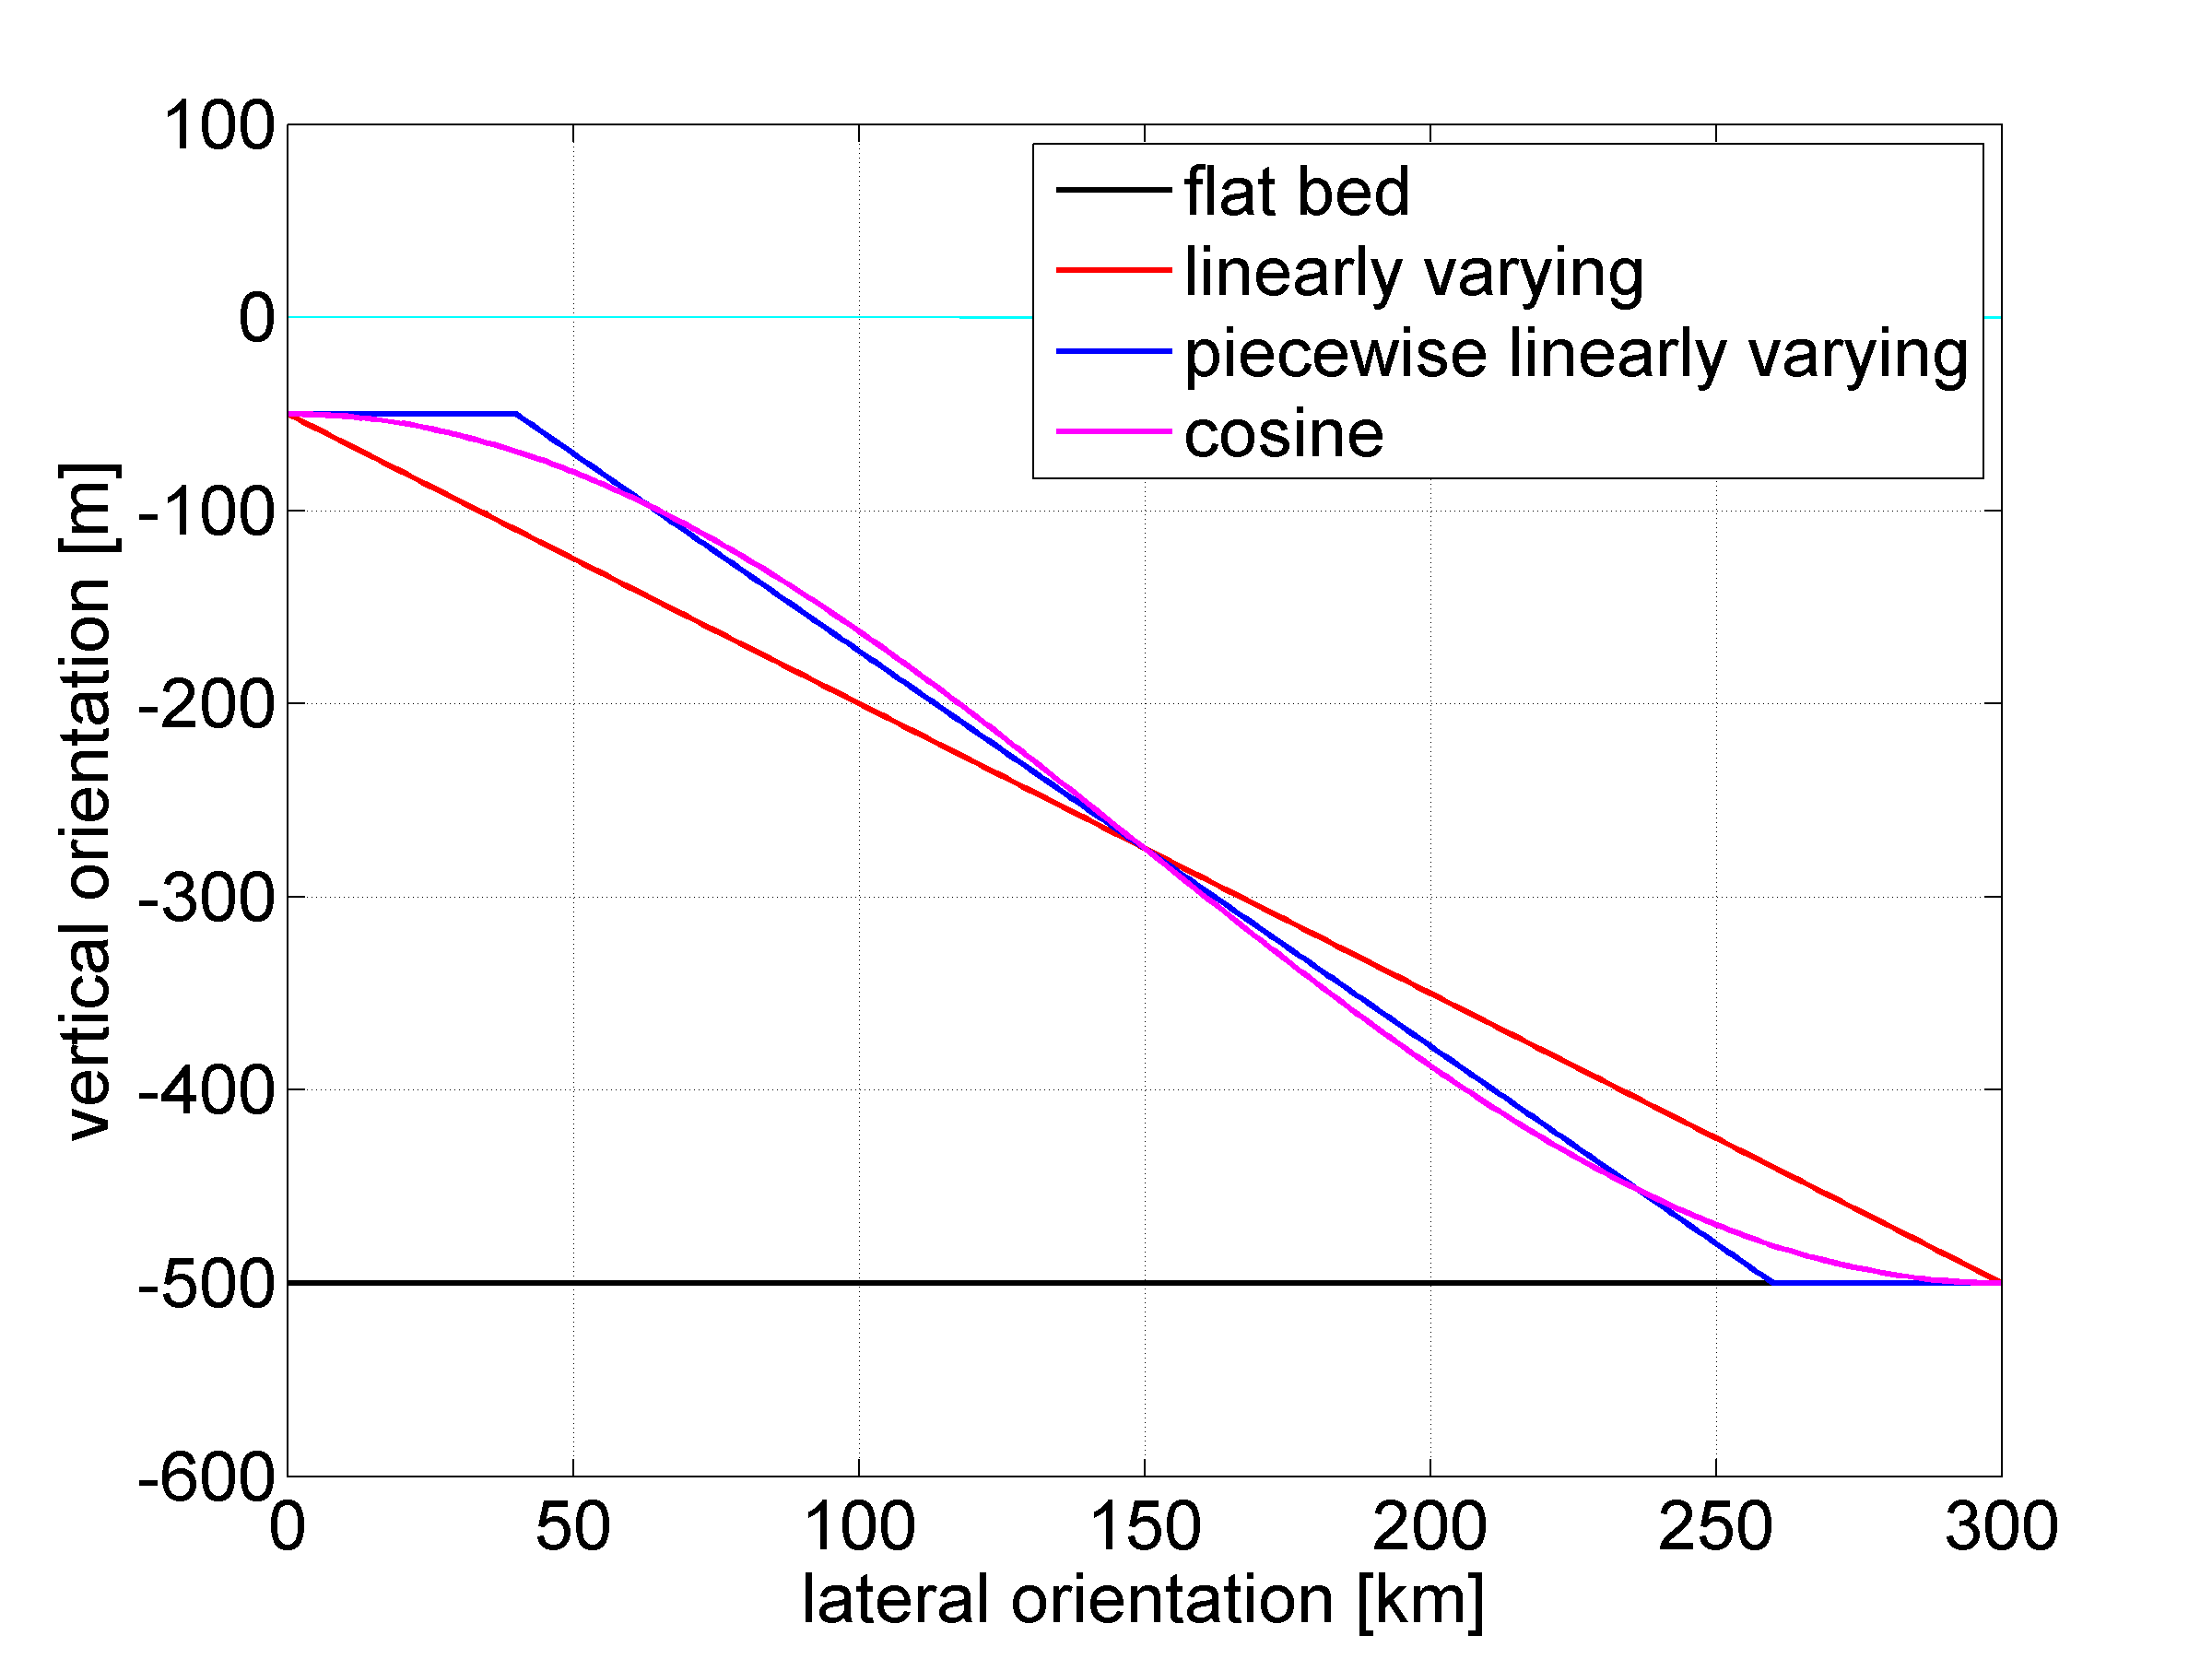
\includegraphics[width=0.55\columnwidth]{figures/coriolisstraightconfig.png}
\end{center}\caption{Various bed level variation approaches for the Coriolis test case. The topography only varies in lateral direction; the bed level is constant in longitudinal (streamwise) direction. \label{fig:coriolisbathymetry}}
\end{figure}

Multiple grids are utilized for this test case. In the basis, distinction is made between grids with quadrilateral cells and with triangular cells. For both types of grids, several grades of refinement are generated.
\begin{figure}[h!]
\begin{center}
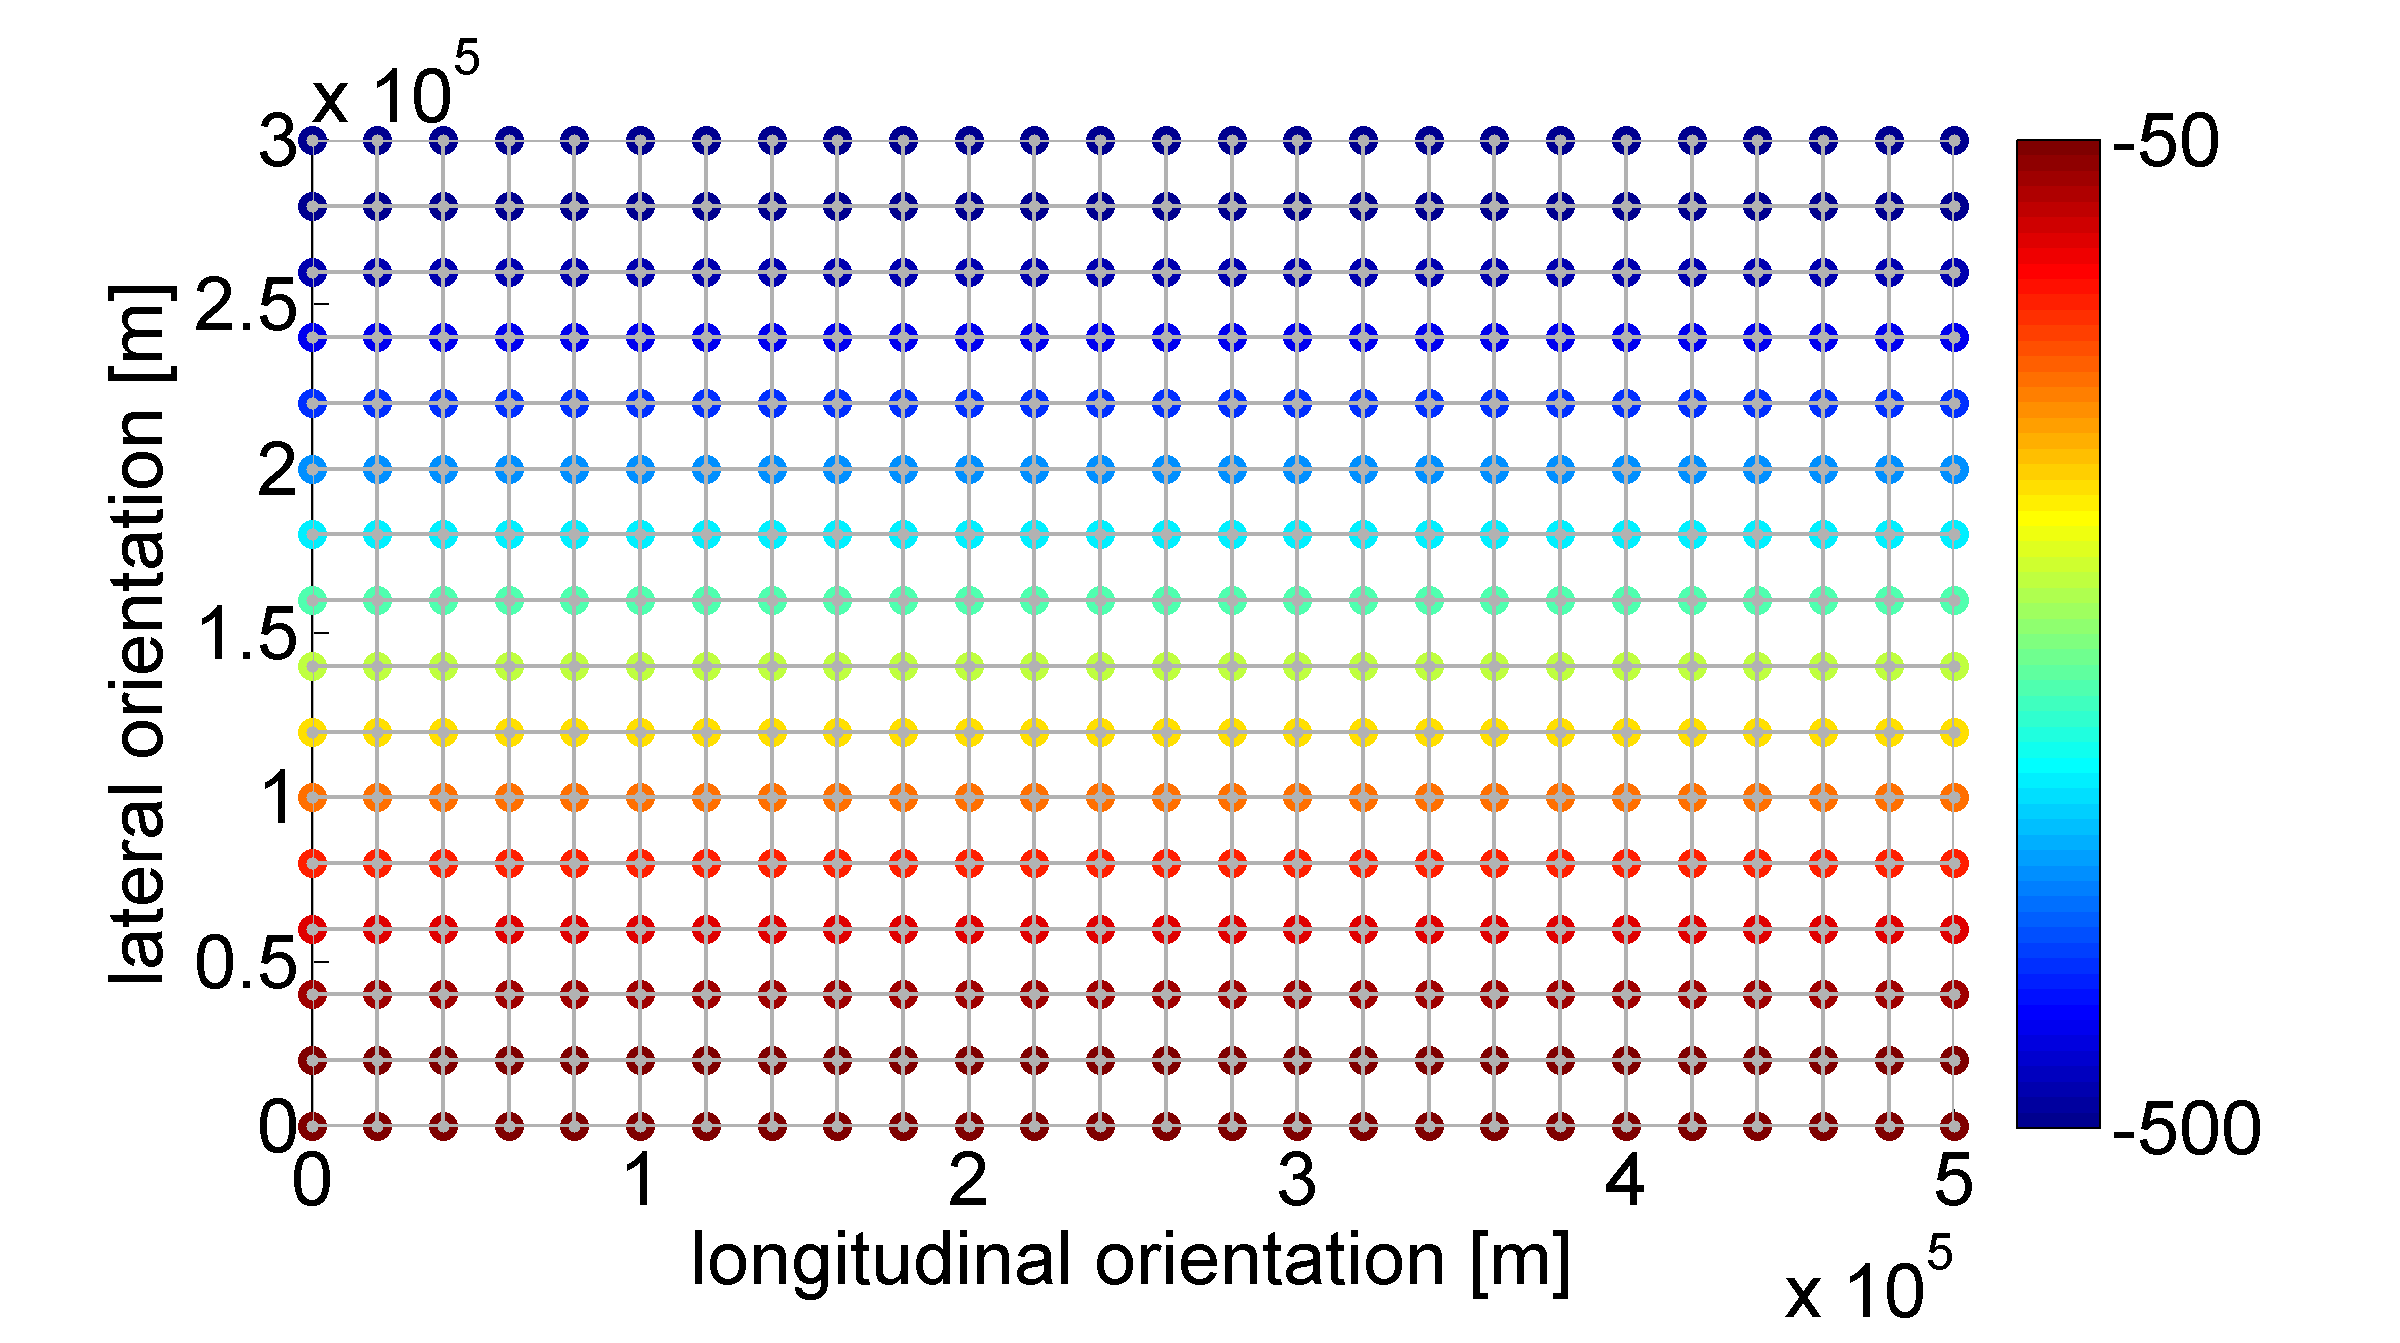
\includegraphics[width=0.48\columnwidth]{figures/coriolisstraightsquares.png}
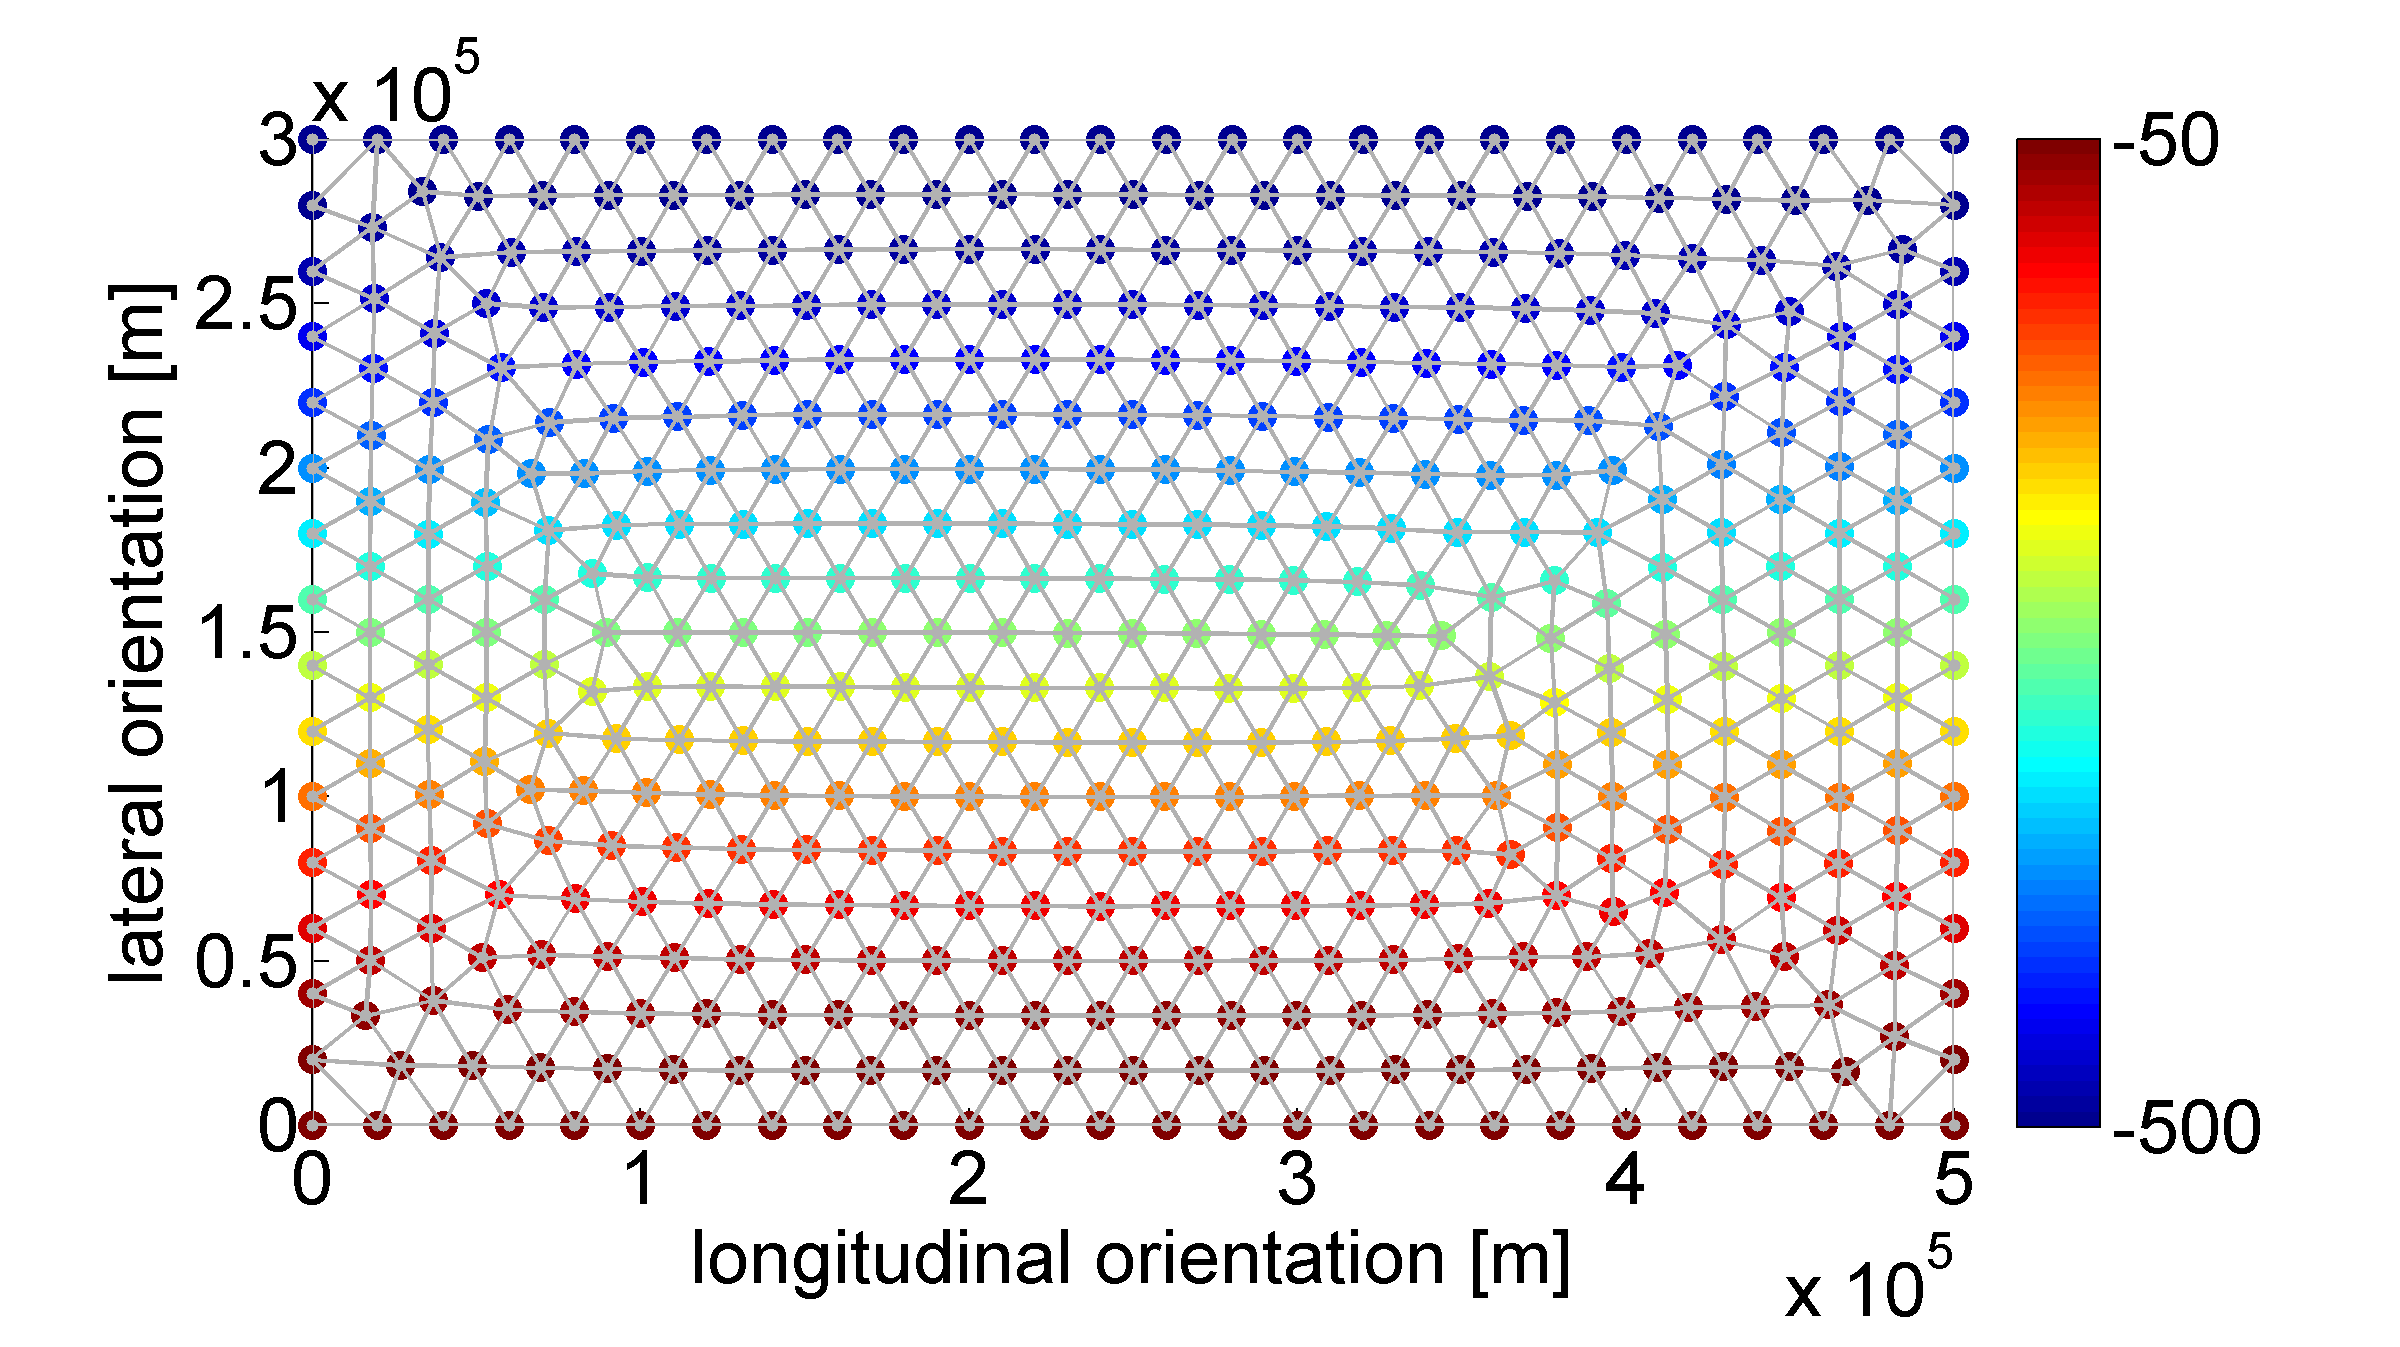
\includegraphics[width=0.48\columnwidth]{figures/coriolisstraighttriangles.png}
\end{center}\caption{Grids used as basis for the test case. Multiple refinement grades are generated as well. The colors indicate the bed level. For the bed level, the cosine-shaped bathymetry is visualized here as an example. \label{fig:coriolisstraightgrids}}
\end{figure}
The refined Cartesian grids are generated by means of refining the grid, shown in the left panel of \Fref{fig:coriolisstraightgrids} once and twice with a factor of 2. The refined triangular grid is generated by means of refining the grid, shown in the right panel of \Fref{fig:coriolisstraightgrids}, once with a factor of 2. The setups shown in \Fref{fig:coriolisstraightgrids} have a cosine-shape for the bed, in lateral direction.





\paragraph*{Results}
In this section, the results are addressed from multiple viewpoints. First, the way of imposing the Riemann invariant is addressed. Second, the effects of grid refinement are investigated for the quadrilateral grids. Third, aspects of the bed level treatment are briefly commented on. Fourth, the grid type (quadrilateral versus triangular) is addressed.

\emph{Spatially varying bathymetry: aspects of prescribing the Riemann invariant}\newline
Prescribing a Riemann invariants invokes the need to know the bed level at the boundary under consideration. Suppose, the gridcell as visualized in \Fref{fig:riemannbndcell} represents a gridcell at the edge of the grid. 
\begin{figure}[h!]
\begin{center}
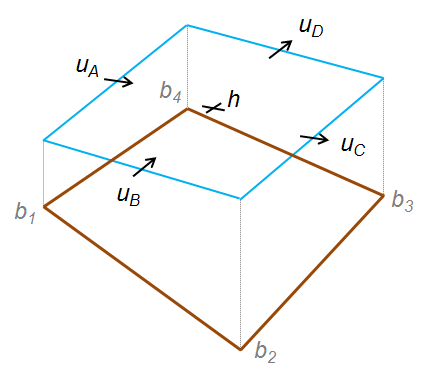
\includegraphics[width=0.3\columnwidth]{figures/computationalcell.png}
\end{center}\caption{Computational cell with surface level $h$, face velocities $u_A$, $u_B$, $u_C$ and $u_D$ and bed levels $b_1$, $b_2$, $b_3$ and $b_4$. \label{fig:riemannbndcell}}
\end{figure}

Think of a boundary at the face with $u_C$ as the face-normal velocity and $b_2$ and $b_3$ as the bed levels along the boundary. The aim is to prescribe the Riemann invariant at the cell center of the ghost-cell outside the boundary, i.e. the mirrored equivalent of the cell shown. As an actual depth, necessary to prescribe the Riemann invariant, the value $(b_2 + b_3)/2$ might be the most intuitive choice.

Two approaches to specify the Riemann invariant are followed and mutually compared:
\begin{enumerate}
\item use $(b_2 + b_3)/2$ for computing the local water depth,
\item use the lowest value, in casu $b_2$, for computing the locat water depth.
\end{enumerate}
The results for both approaches are visualized in \Fref{fig:resultscoriolisbathymetry} for each bathymetry (flat bed, linear bed, piecewise linear bed and cosinal bed). Notice that for the flat bed, no effect of either the one choice or the other is expected (constant depth). Moreover, notice that taking the lowest bed level is equivalent to shift the Riemann boundary data series along the boundary over half a grid cell.

\begin{figure}[h!]
\begin{center}
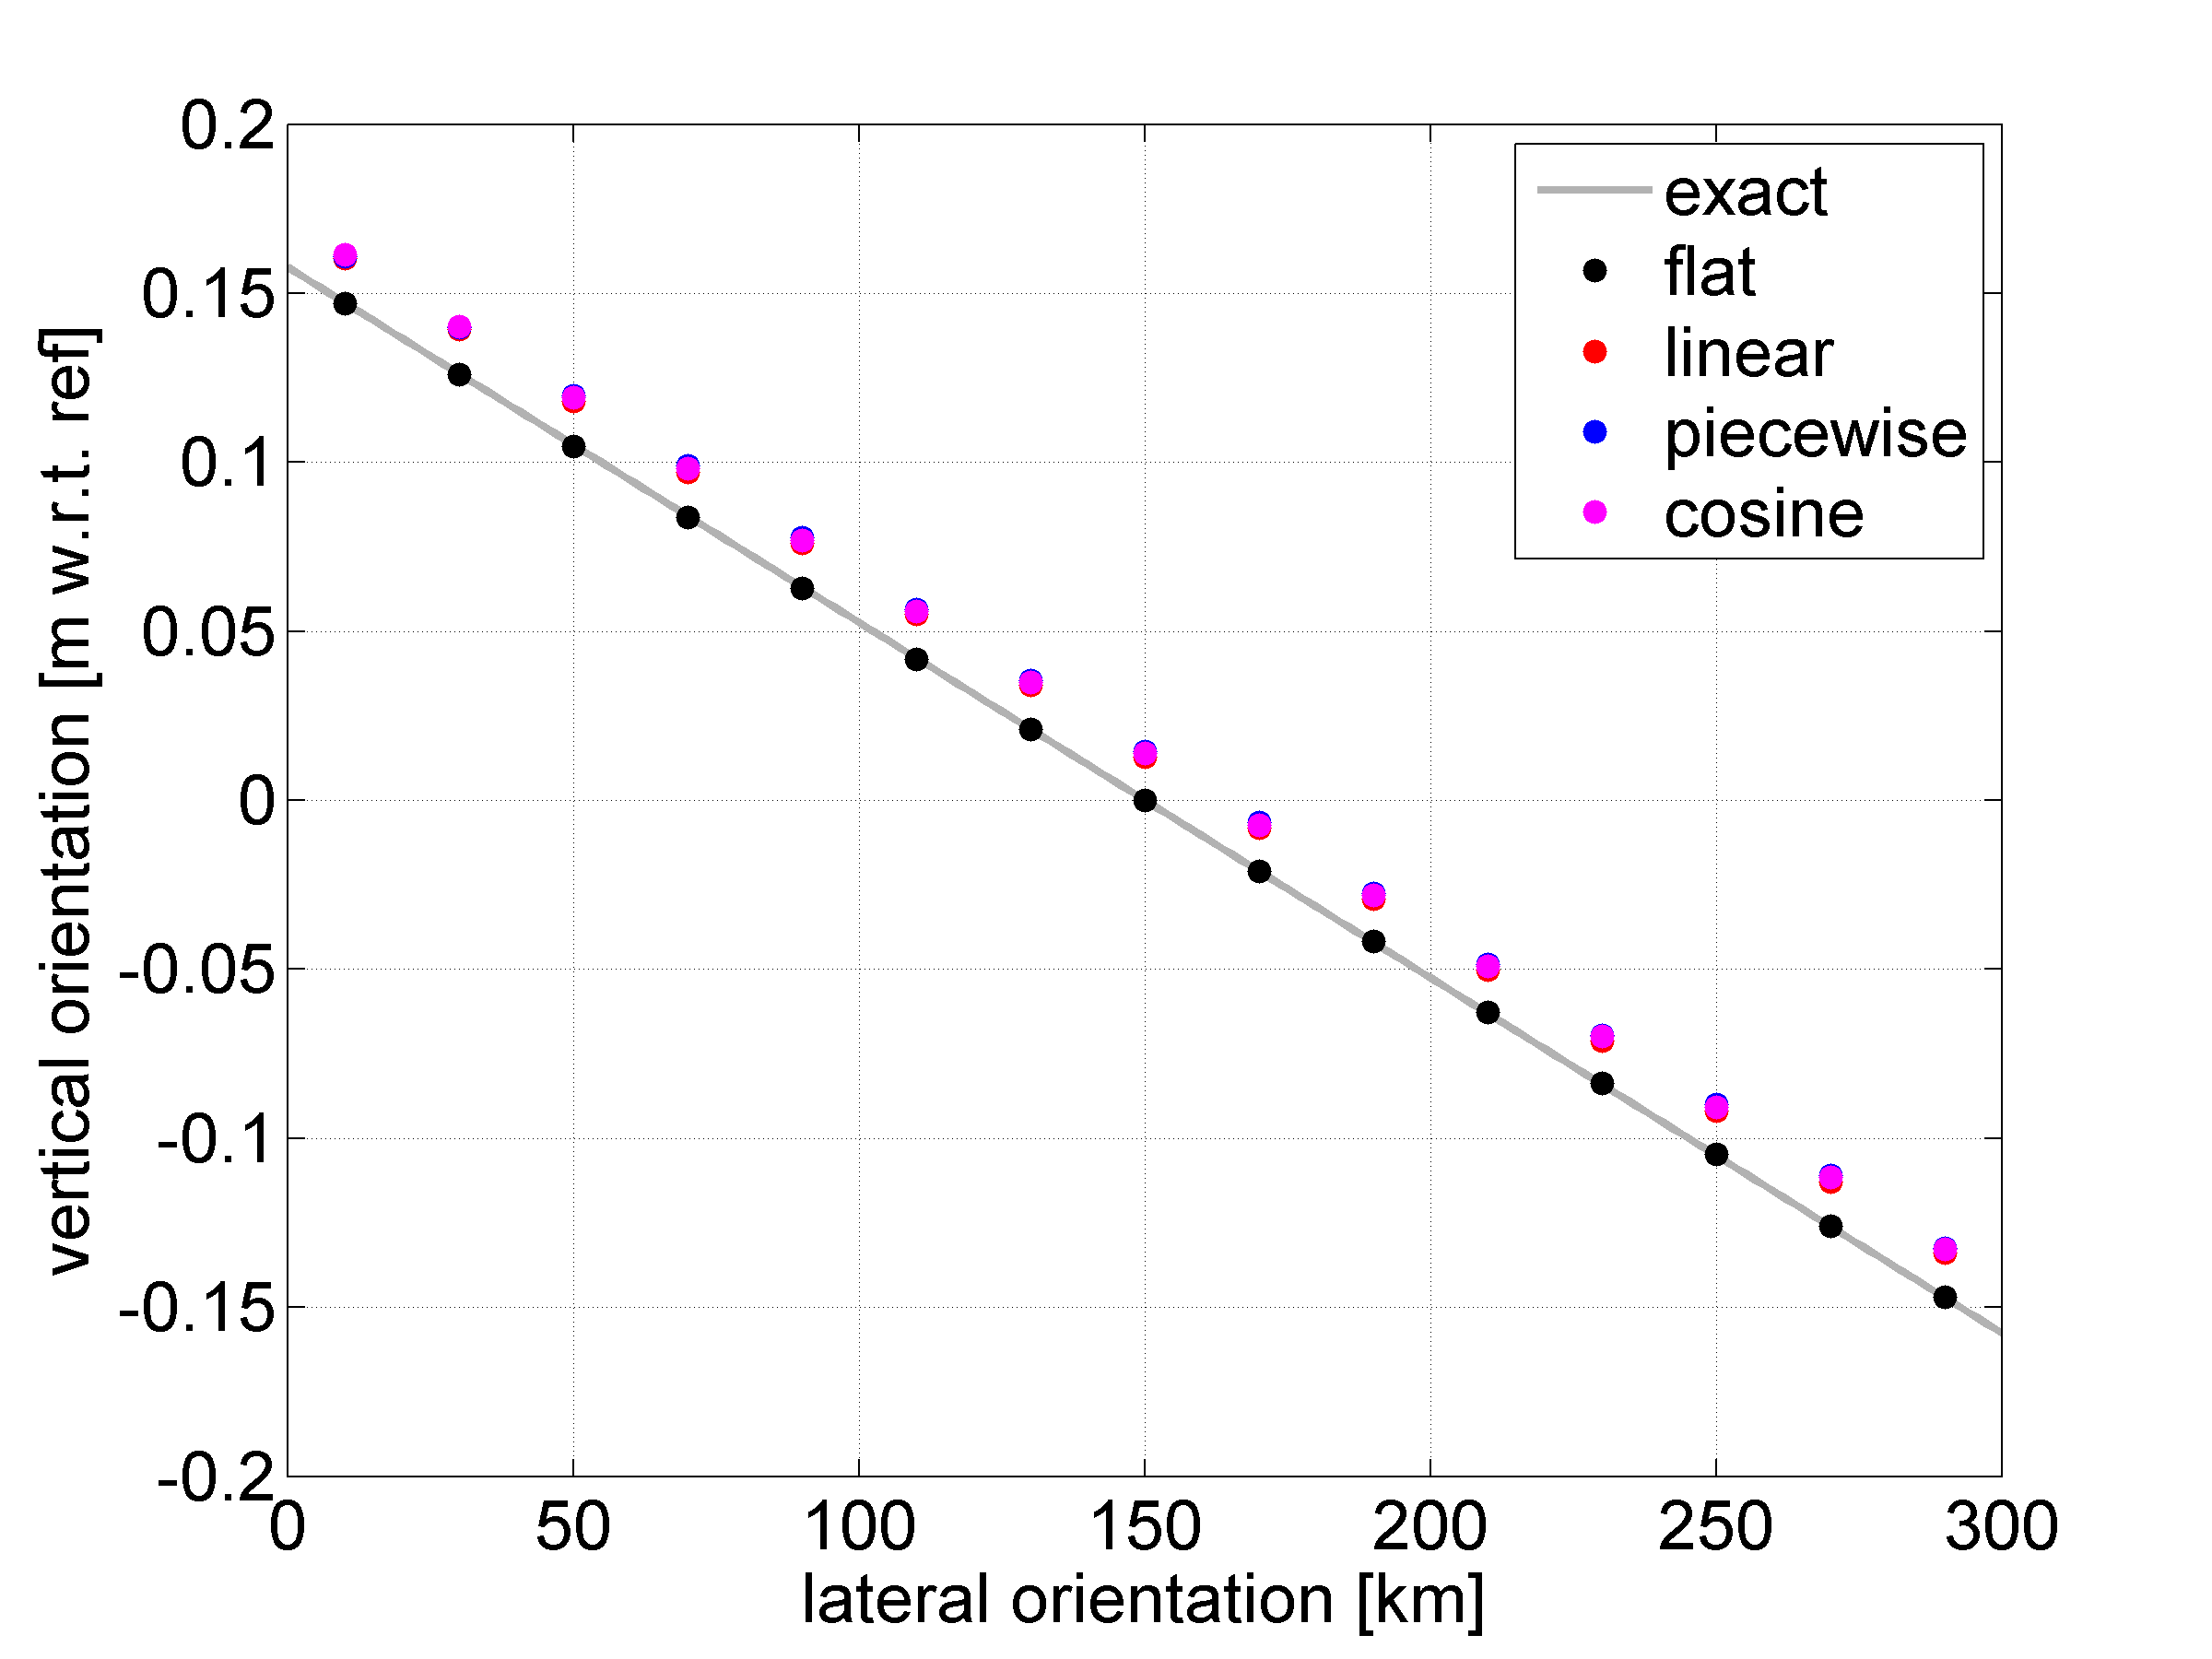
\includegraphics[width=0.48\columnwidth]{figures/resultsbathymetry.png}
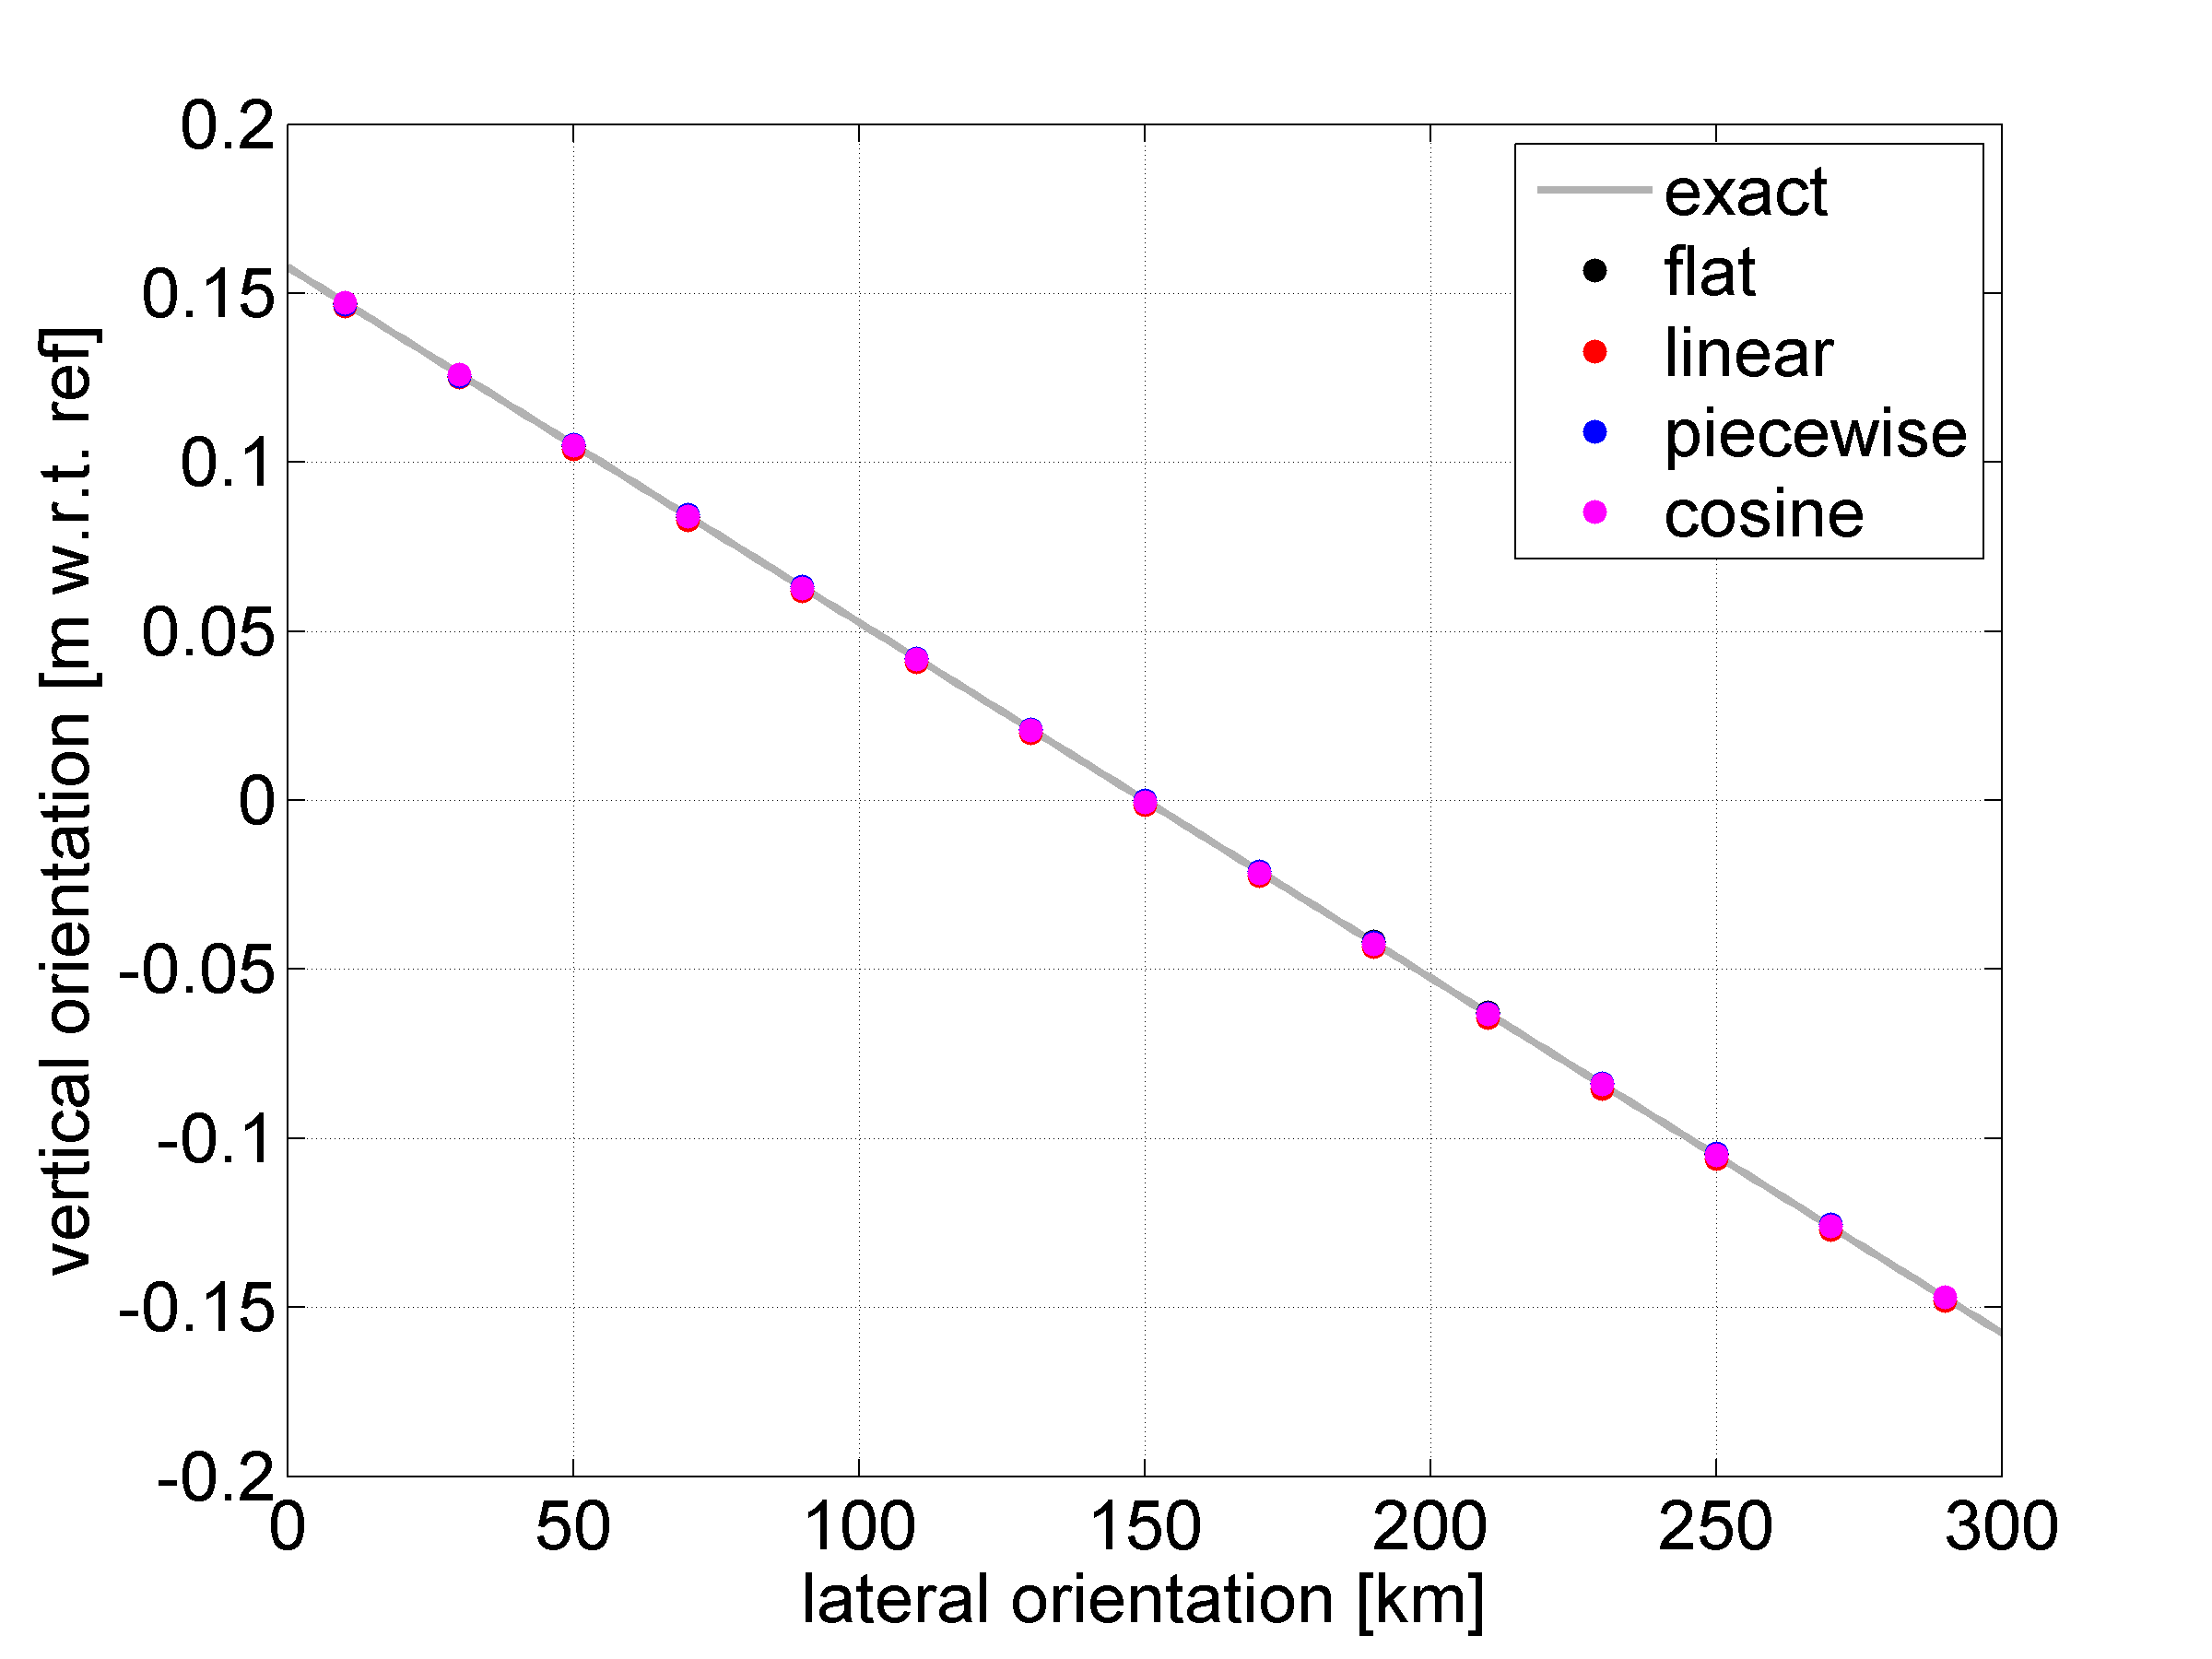
\includegraphics[width=0.48\columnwidth]{figures/resultsbathymetryshift.png}
\end{center}\caption{Numerical solution for the various bathymetry configuration in relation to the exact solution. Left panel: standard way of imposing a Riemann invariant; right panel: with a Riemann invariant, imposed with a shift of half a gridcell. \label{fig:resultscoriolisbathymetry}}
\end{figure}

The results, shown in \Fref{fig:resultscoriolisbathymetry}, show that taking the lowest bed level for the computation of the local water depth returns a good result, whereas this is not the case for the approach in which we use the mean bed level. For all the bathymetry configurations, the results coincide.


\emph{Spatially varying bathymetry: aspects of the bed level treatment}\newline
For the treatment of the bed level (cf. \Fref{fig:riemannbndcell}), the user can use the mdu-keywords \texttt{conveyance2d} and \texttt{bedlevtyp} to make D-Flow FM handle according to the user's demands. In order to explore the effects of the joint choice for both keywords, the options \texttt{conveyance2d = -1/3} and the options \texttt{bedlevtyp = 1/2/3/4/5} are varied in all possible combinations.

The results of these additional computations are as follows:
\begin{itemize}
\item the options \texttt{bedlevtyp = 1/2} returned poor results, regardless of the choice for \texttt{conveyance2d},
\item the options \texttt{bedlevtyp = 3/4/5} returned mutual differences that are of an order of magnitude smaller than the difference with the exact solution as shown in the left panel of \Fref{fig:resultscoriolisbathymetry}, regardless of the choice for \texttt{conveyance2d}.
\end{itemize}





\emph{Flat bathymetry: effects of grid refinement}\newline
The flat bed case is used for a grid convergence study. For this purpose, only the three Cartesian grids are considered: the first with cells with an edge length of 20~km, the second 10~km and the third 5~km. The differences with the exact solution are measured with an $L_2$-norm. For each simulation, the timestep $\Delta t = 50$~seconds is chosen. The simulations cover 10 days of simulated time, which has proven to be sufficient to reach a steady state. 

The $L_2$-norm of the difference between the exact solution and the numerical solution is shown in \Fref{fig:resultscoriolisconvergence} against the typical grid cell size. \Fref{fig:resultscoriolisconvergence} reveals zeroth order convergence of the $L_2$-norm measure.

\begin{figure}[h!]
\begin{center}
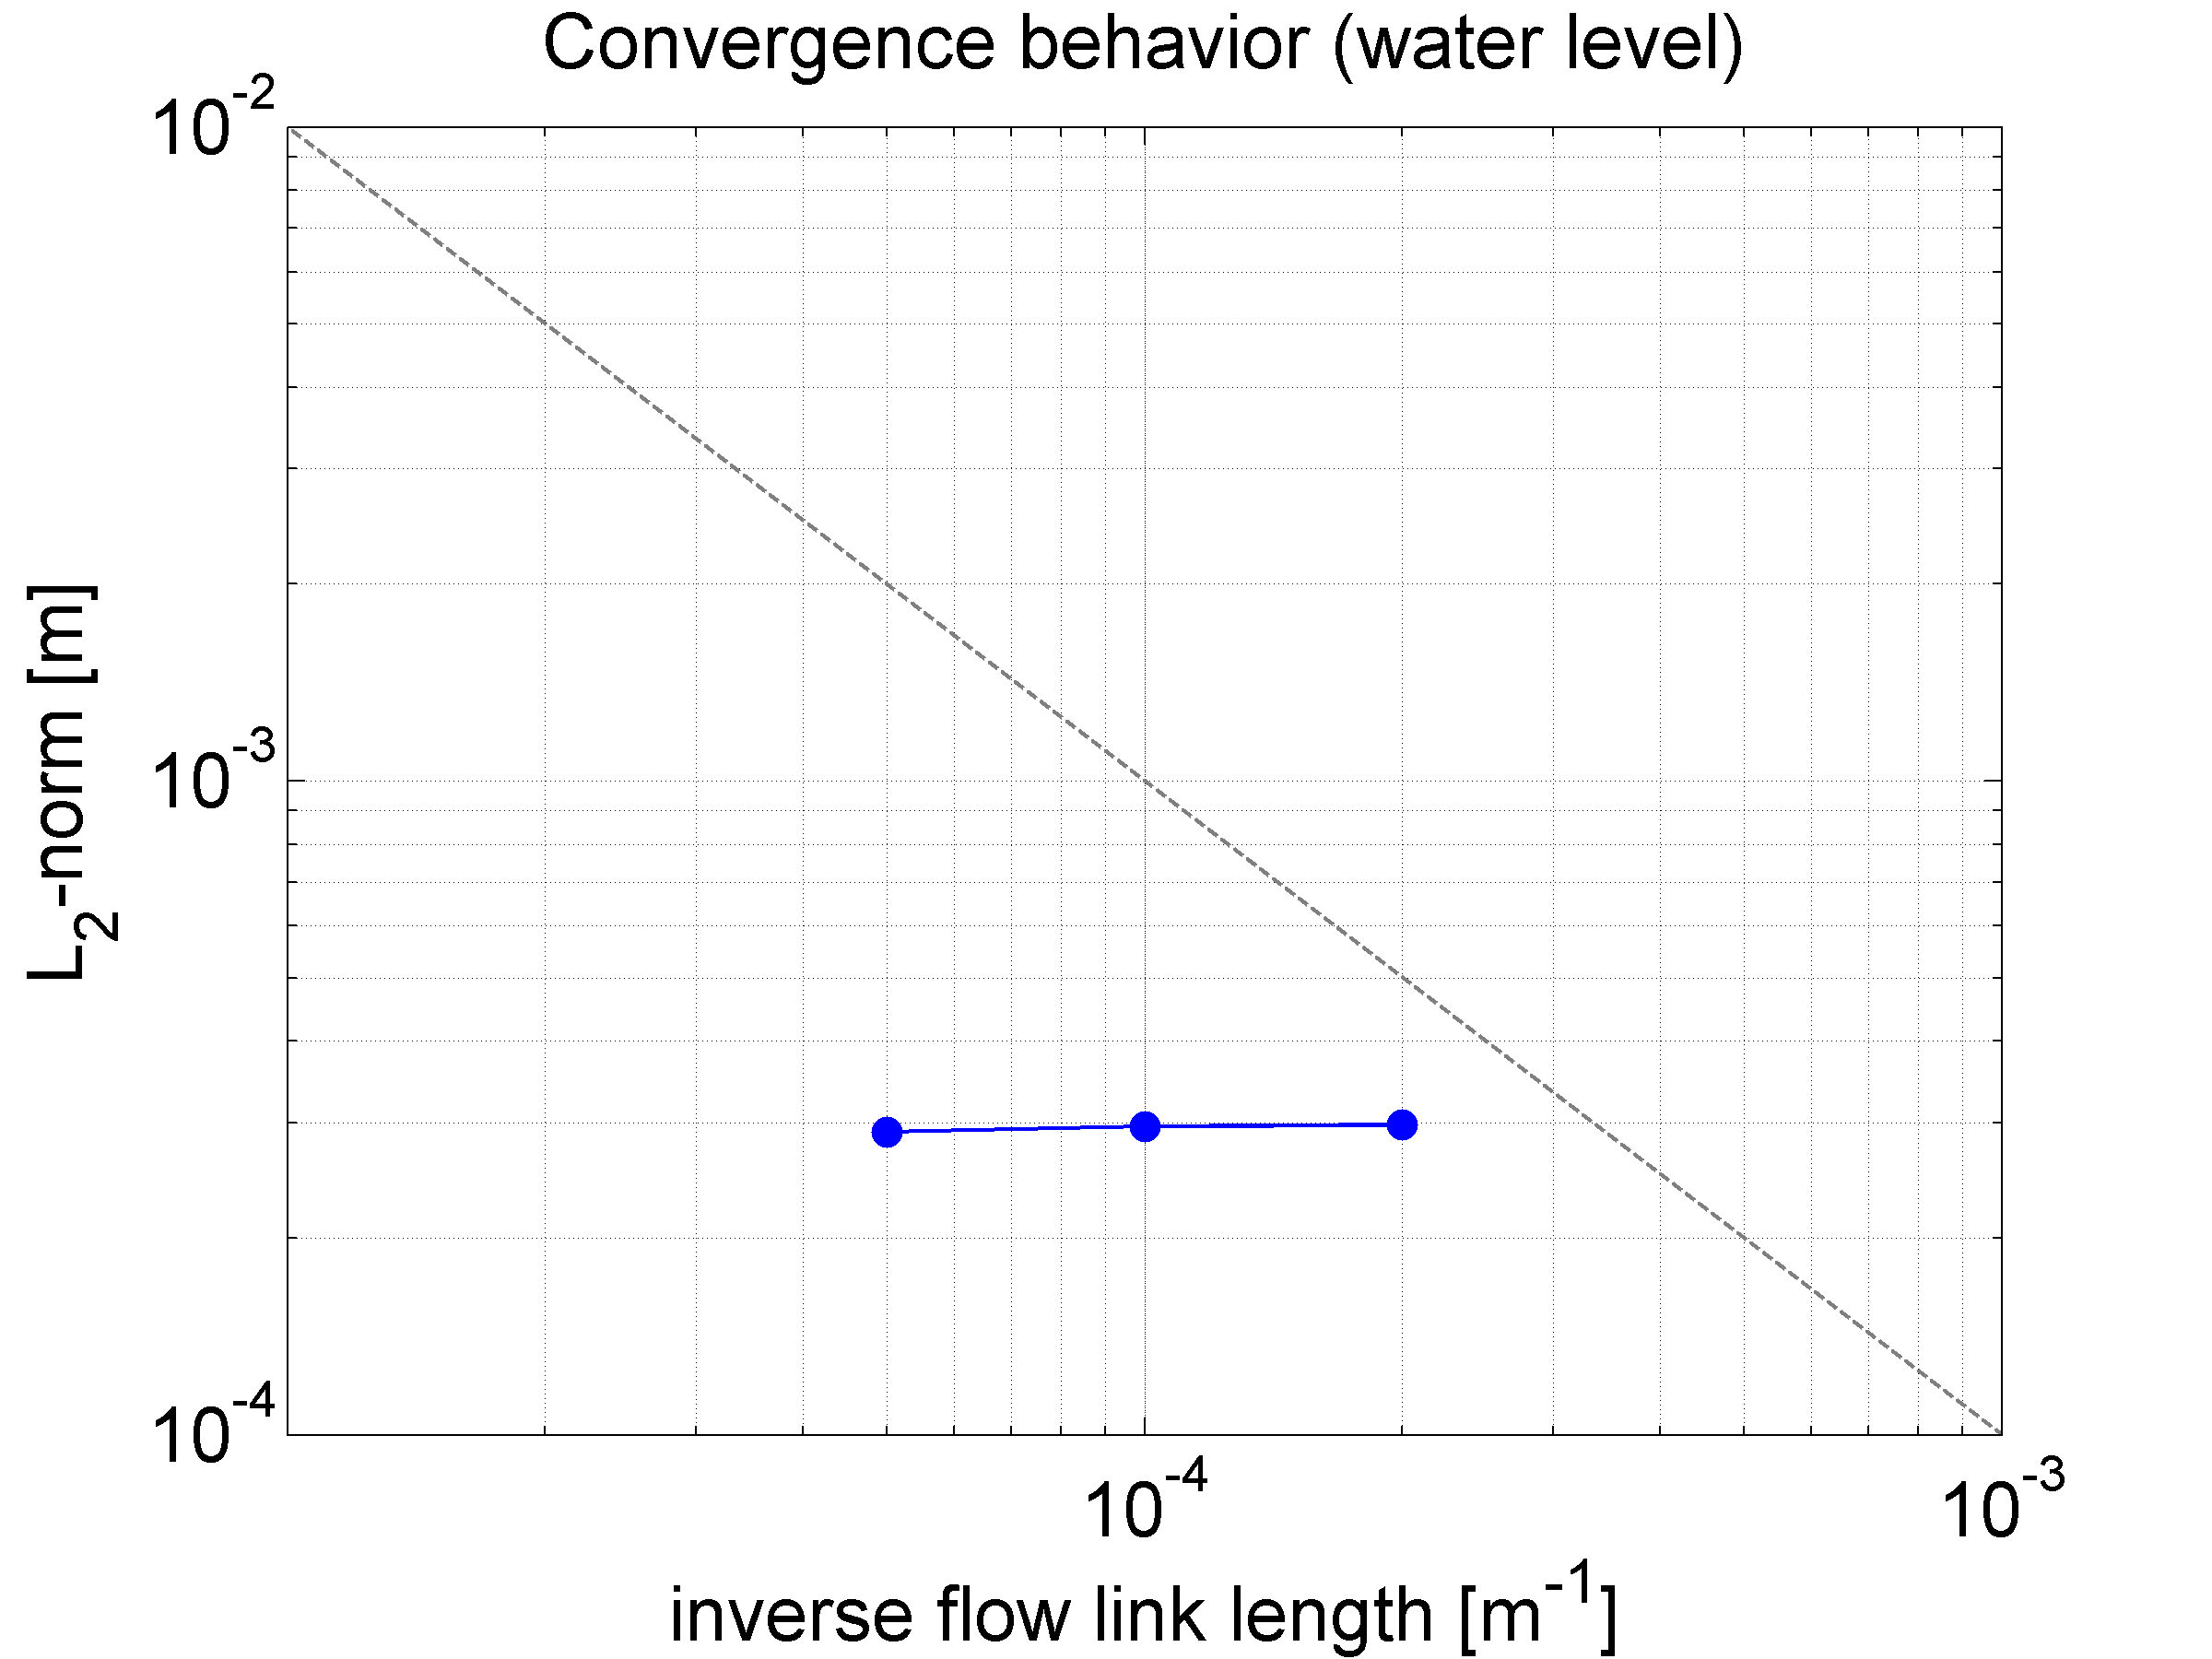
\includegraphics[width=0.55\columnwidth]{figures/coriolisstraightconvergence.png}
\end{center}\caption{Convergence behavior of the $L_2$-norm of the water level difference (the numerical solution minus the exact solution). The dashed line represents first order behavior. \label{fig:resultscoriolisconvergence}}
\end{figure}





\emph{On the type of the grid: quadrilateral or triangular cells}\newline
The simulations for the flat bed setup and the cosine bed setup have been conducted on both a quadrilateral (or Cartesian) grid and a triangular grid. This enables a comparison of the accuracy of both approaches. Using the $L_2$-norm of the differences between the exact water levels and the computed water levels, the results read:
\begin{itemize}
\item Flat bed bathymetry on a Cartesian grid: 2.963195095572729e-04 m,
\item Flat bed bathymetry on a triangular grid: 4.813599995505768e-02 m,
\item Cosine shaped bathymetry on a Cartesian grid: 1.405800785225406e-02 m,
\item Cosine shaped bathymetry on a triangular grid: 8.379261007472463e-03 m.
\end{itemize}
For the flat bed case, the triangular grid returns less accurate results compared to the quadrilateral grid. For the cosine shaped bathymetry case, the opposite appears to hold. Hence, no clear general conclusion can be drawn on the basis of these results.





\paragraph*{Conclusion}
From the above considerations, the following conclusions can be drawn:
\begin{itemize}
\item D-Flow FM is able to reproduce the analytical solution for the balance between the Coriolis force and the slope of the water surface in a long straight channel, regardless of the bathymetry shape,
\item the way of prescribing a Riemann invariant at the outflow boundary could be perceived of as confusing regarding the value of the bed level to use for the water depth definition,
\item for the flat bed case, zeroth order convergence behavior is measured for the computed water level with decreasing grid cell size,
\item no clear conclusion can be drawn regarding the accuracy of quadrilateral grids versus triangular grids.
\end{itemize}



\paragraph*{Version}
This test has been carried out with version dflow-fm-x64-1.1.136.39235.



